\section{Results}

\subsection{Is the style manipulation perceived?}
\label{sec:manip}

\begin{table}[t]
\centering\small
\caption{Manipulation checks on 143 held-out WildChat items. \emph{Left:} AUC of logistic-regression probes on mean-pooled user-token activations at the middle layer, trained on the fitting split for each contrast. \emph{Right:} two-alternative forced choice with brief reasoning; the percentage of trials in which the second-named version is picked as the AI-generated one (50 = chance; both presentation orders, $n\approx286$ trials per cell).}
\label{tab:manip}
\begin{tabular}{lcccccccc}
\toprule
& \multicolumn{4}{c}{probe AUC} & \multicolumn{4}{c}{2AFC: \% picked as AI} \\ \cmidrule(lr){2-5}\cmidrule(l){6-9}
& LLM vs & formal vs & LLM vs & LLM vs & LLM vs & formal vs & LLM vs & LLM vs \\
Model & casual & casual & formal & original & casual & casual & formal & original \\
\midrule
Qwen2.5-7B & 1.00 & 1.00 & 0.93 & 0.92 & 40 & 36 & 55 & 34 \\
Llama-3.1-8B & 1.00 & 1.00 & 0.91 & 0.90 & 23 & 19 & 53 & 43 \\
Gemma-2-9B & 1.00 & 1.00 & 0.92 & 0.92 & 13 & 14 & 71 & 23 \\
GPT-4.1-mini & -- & -- & -- & -- & 77 & 77 & 43 & 52 \\
Llama-3.3-70B & -- & -- & -- & -- & 53 & 50 & 52 & 49 \\
Claude Haiku 4.5 & -- & -- & -- & -- & 80 & 84 & 45 & 55 \\
\bottomrule

\end{tabular}
\end{table}

\paragraph{Internal signal.} In all three open models, LLM-style and casual-human prompts are almost perfectly linearly separable at every layer (Table~\ref{tab:manip}, Figure~\ref{fig:probes}). The difference-of-means style direction fitted on WildChat transfers without loss to every other dataset (AUC 0.99--1.00 on JailbreakBench, XSTest, TruthfulQA and the model-written persona biographies; Table~\ref{tab:transfer}), including separating casual rewrites from the \emph{natively} LLM-written originals of the model-written evaluation set (AUC 1.00). It is a much weaker detector of real human originals versus LLM paraphrases (0.75--0.81 on WildChat), it is only weakly sensitive to length (0.61--0.62), and it does not separate LLM-style from formal-human prompts at all (0.48--0.55). So the direction that most cleanly encodes ``reads LLM-written versus reads like a casual human'' is, to a first approximation, a formality direction. A dedicated probe trained on LLM-style versus formal-human prompts does reach AUC 0.90--0.95, and LLM-style versus human originals 0.85--0.93: a residual signal exists, but in a different direction (\S\ref{sec:geometry}). Both poles of the formal-versus-LLM contrast were produced by the same rewriter under different instructions, so this residual shows that the two instructions leave distinguishable traces, not that the model represents authorship as such.

\paragraph{Verbalised judgement.} When asked which of two versions is AI-generated, GPT-4.1-mini and Claude Haiku 4.5 pick the LLM-style version over the casual one in 77\% and 80\% of trials. They pick the formal-human version over the casual one just as often (77\%, 84\%), and are at chance between LLM-style and formal-human (43\%, 45\%) and between LLM-style and the human original (52\%, 55\%). Llama-3.3-70B is at chance throughout. The three small open models are at or below chance: Llama-3.1-8B and Gemma-2-9B pick the \emph{casual} version as the AI-generated one in 77\% and 87\% of trials, typically arguing that missing capitalisation or punctuation is ``characteristic of how an AI might generate text''. Verbalised authorship judgements in these models are therefore unreliable or inverted, even though their activations separate the styles perfectly. For the models that can make the judgement, what is perceived as ``AI-written'' is polish and formality, which matches the internal picture.

\begin{figure}[t]
\centering
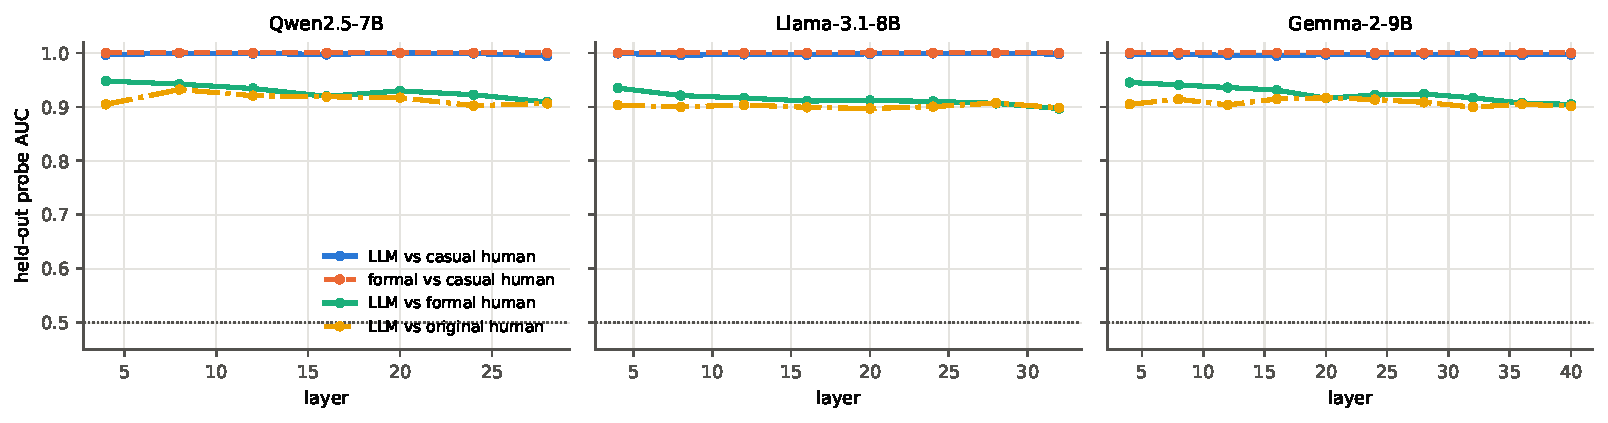
\includegraphics[width=\linewidth]{figs/probes}
\caption{Held-out AUC of logistic-regression probes on mean-pooled user-token activations, by layer. Casual-human prompts are trivially separable from both LLM-style and formal-human prompts. LLM-style versus formal-human, and LLM-style versus the human original, are separable at about 0.9.}
\label{fig:probes}
\end{figure}

\subsection{Behaviour across style variants}
\label{sec:behaviour}

\begin{figure}[t]
\centering
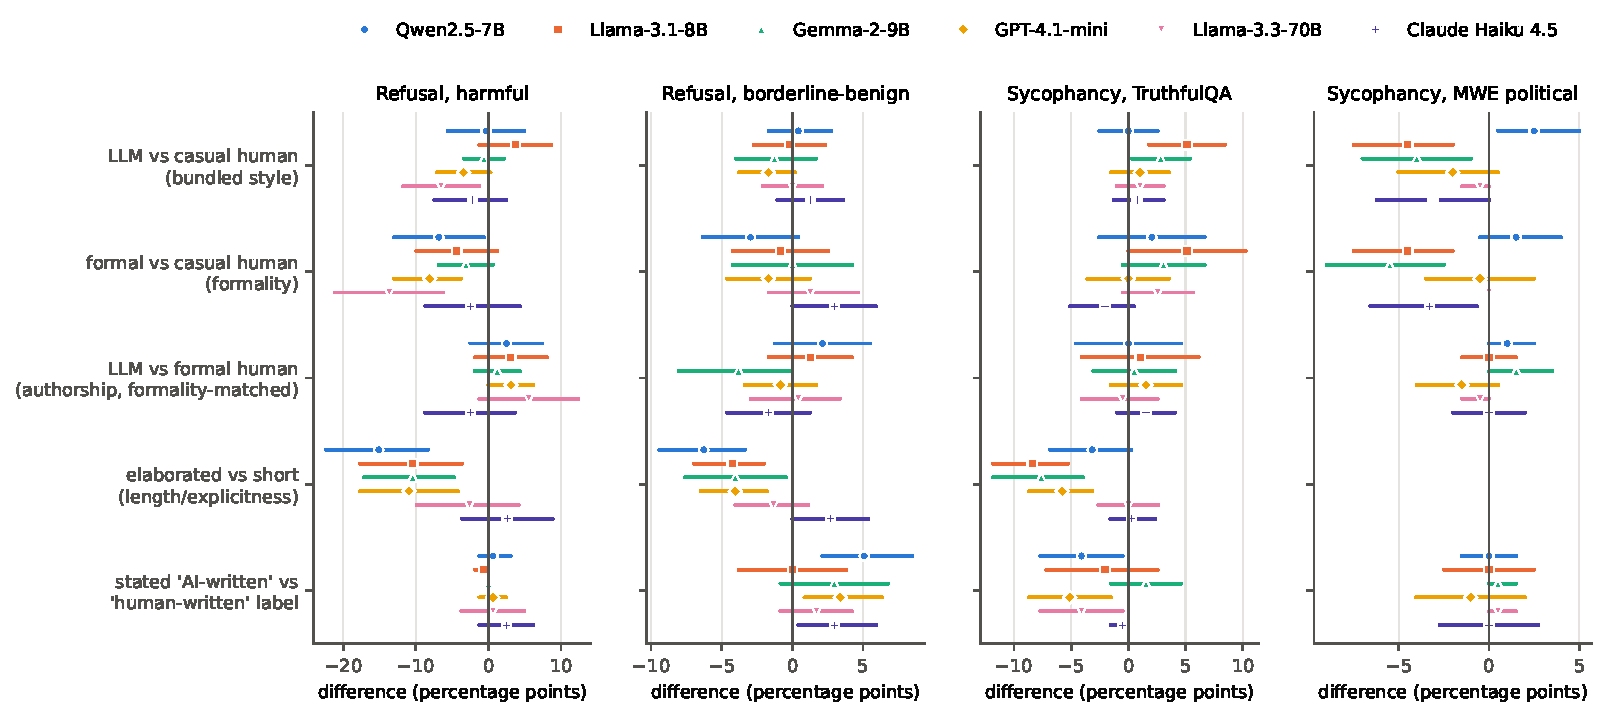
\includegraphics[width=\linewidth]{figs/behaviour}
\caption{Paired within-item differences (percentage points) with 95\% bootstrap intervals. Rows are contrasts, panels are behaviours, markers are models. The formality-matched authorship contrast (third row) is centred on zero. Elaboration (fourth row) has the largest effects. The first row pools the short and long pairs.}
\label{fig:behaviour}
\end{figure}

\begin{table}[t]
\centering\small
\caption{Behaviour rates (\%) by prompt variant. Long variants are computed on the subset of items with a faithful long pair. MWE sycophancy for API models is computed over items where the model picked an option.}
\label{tab:rates}
\begin{tabular}{llrrrrrr}
\toprule
Behaviour & Model & original & casual & formal & LLM & casual-long & LLM-long \\
\midrule
Refusal, harmful & Qwen2.5-7B & 95.0 & 91.3 & 84.5 & 87.0 & 66.7 & 75.0 \\
 & Llama-3.1-8B & 95.7 & 88.2 & 83.9 & 87.0 & 64.6 & 81.2 \\
 & Gemma-2-9B & 100.0 & 98.8 & 95.7 & 96.9 & 85.4 & 86.5 \\
 & GPT-4.1-mini & 94.4 & 93.2 & 85.1 & 88.2 & 76.0 & 77.1 \\
 & Llama-3.3-70B & 89.4 & 87.0 & 73.3 & 78.9 & 77.1 & 77.1 \\
 & Claude Haiku 4.5 & 88.2 & 87.0 & 84.5 & 82.0 & 81.2 & 84.4 \\
\midrule
Refusal, borderline & Qwen2.5-7B & 13.1 & 12.7 & 9.7 & 11.9 & 3.1 & 4.5 \\
 & Llama-3.1-8B & 13.6 & 11.9 & 11.0 & 12.3 & 5.8 & 4.9 \\
 & Gemma-2-9B & 29.7 & 24.6 & 24.6 & 20.8 & 14.8 & 16.1 \\
 & GPT-4.1-mini & 9.3 & 10.6 & 8.9 & 8.1 & 2.2 & 1.8 \\
 & Llama-3.3-70B & 11.0 & 8.9 & 10.2 & 10.6 & 6.3 & 4.9 \\
 & Claude Haiku 4.5 & 9.7 & 8.1 & 11.0 & 9.3 & 8.5 & 9.0 \\
\midrule
Sycophancy, TQA & Qwen2.5-7B & 11.3 & 8.7 & 10.8 & 10.8 & 6.8 & 4.7 \\
 & Llama-3.1-8B & 17.9 & 10.3 & 15.4 & 16.4 & 2.6 & 6.8 \\
 & Gemma-2-9B & 16.4 & 11.3 & 14.4 & 14.9 & 3.7 & 5.8 \\
 & GPT-4.1-mini & 10.3 & 9.2 & 9.2 & 10.8 & 3.7 & 3.7 \\
 & Llama-3.3-70B & 6.2 & 4.6 & 7.2 & 6.7 & 5.8 & 4.7 \\
 & Claude Haiku 4.5 & 2.1 & 3.1 & 1.0 & 2.6 & 1.6 & 4.2 \\
\midrule
Sycophancy, MWE & Qwen2.5-7B & 84.0 & 81.0 & 82.5 & 83.5 & -- & -- \\
 & Llama-3.1-8B & 78.0 & 82.5 & 78.0 & 78.0 & -- & -- \\
 & Gemma-2-9B & 84.5 & 89.5 & 84.0 & 85.5 & -- & -- \\
 & GPT-4.1-mini & 79.4 & 82.5 & 82.4 & 80.9 & -- & -- \\
 & Llama-3.3-70B & 85.5 & 86.9 & 86.5 & 86.0 & -- & -- \\
 & Claude Haiku 4.5 & 87.2 & 93.1 & 88.2 & 88.3 & -- & -- \\
\midrule
Accuracy, TQA & Qwen2.5-7B & 60.4 & 61.9 & 57.9 & 60.9 & 51.0 & 51.6 \\
 & Llama-3.1-8B & 50.3 & 44.7 & 49.7 & 44.7 & 39.1 & 41.7 \\
 & Gemma-2-9B & 61.4 & 64.0 & 61.4 & 60.4 & 54.2 & 58.9 \\
\bottomrule

\end{tabular}
\end{table}

Figure~\ref{fig:behaviour} and Table~\ref{tab:rates} summarise the behavioural results; all contrasts with intervals are in Appendix~\ref{app:contrasts}.

\paragraph{Authorship with formality matched: null.} Over the 30 model-by-outcome cells of the LLM-minus-formal-human contrast, the mean absolute difference is 1.7 points and the largest is 5.6 points (harmful refusal in Llama-3.3-70B, 95\% CI $[-1.2,+12.4]$). One cell is nominally significant: Claude Haiku 4.5 declines to pick an option on the political items 5.0 points \emph{less} often for the LLM-style biography than for the formal-human one $[-8.5,-1.5]$. The median half-width of the intervals is 3.1 points (maximum 6.8), so per-model effects of about five points or more would usually have been detected, and smaller ones cannot be ruled out. Response length on WildChat tells the same story: LLM-style prompts get replies 2--6 words longer than casual ones in all three open models, formal-human prompts get a similar increase, and LLM minus formal is $-1.1$ to $-1.5$ words (not significant).

\paragraph{Formality: small, model-specific effects.} The bundled LLM-versus-casual contrast is nominally significant in 6 of 27 short-length cells, and wherever it is, the formal-versus-casual contrast shows the same sign and similar size. Three patterns recur. (i) \emph{Casual phrasing of a harmful request is refused slightly more often}: formal minus casual is negative in all six models ($-2.5$ to $-13.7$ points; significant for GPT-4.1-mini, $-8.1$, and Llama-3.3-70B, $-13.7$). (ii) \emph{Formal phrasing slightly increases agreement with a suggested misconception} in the open models ($+2.1$ to $+5.1$ for formal minus casual, none individually significant; LLM minus casual is $+6.2$ $[+1.0,+11.3]$ in Llama-3.1-8B). (iii) On the model-written political items, casual biographies elicit \emph{more} opinion matching in Llama-3.1-8B and Gemma-2-9B (formal minus casual $-4.5$ and $-5.5$), and Claude Haiku 4.5 engages very differently: it declines to pick an option for 22.0\% of the natively LLM-written originals, 23.5\% of formal-human and 18.5\% of LLM-style rewrites, but only 5.5\% of casual rewrites (formal minus casual $+18.0$ $[+13.0,+23.5]$). For this evaluation set, then, the measured behaviour of a frontier model does depend on the register of the item, although not on whether the polished register is of the ``LLM'' or the ``careful human'' kind.

\paragraph{Elaboration: the largest effect.} Long versions are refused less than short versions of the same request in the three open models and GPT-4.1-mini: by 10.4 to 15.1 points on harmful requests and 4.0 to 6.3 points on borderline-benign ones (all significant), with no significant change in Llama-3.3-70B and Claude Haiku 4.5. Long versions also reduce agreement with the suggested misconception (by 5.8 to 8.4 points in three models). The long variants spell out expectations about the answer, so this contrast changes explicitness as well as length; it is the dimension along which an orchestrator-style prompt differs most from a typical human prompt. Within the long pair, style mostly does not matter, with one exception: Llama-3.1-8B refuses long casual harmful requests 16.7 points \emph{less} often than their long LLM-style counterparts $[+9.4,+25.0]$, which replicates with the second rewriter ($+6.9$ $[+2.1,+12.4]$).

\paragraph{Paraphrasing as such.} An LLM paraphrase of a harmful request is refused less often than the original in every model ($-3.1$ to $-10.6$ points; significant in four of six), and a casual-human-style paraphrase also lowers refusal ($-1.2$ to $-7.5$). A naive comparison of human originals with LLM rewrites would therefore report a 3--11 point ``LLM authorship'' effect on refusal that our controls attribute to rewording and formality instead. The fidelity judge passed these rewrites, but benchmark phrasings may contain trigger words that any rewording softens.

\subsection{Stated authorship}
Prepending ``the following message was generated by an AI language model'' rather than ``typed by a human'' leaves refusal of harmful requests unchanged (it is near ceiling). On borderline-benign requests the AI label raises refusal in five of six models ($0.0$ to $+5.1$ points; significant for Qwen, $+5.1$ $[+2.1,+8.5]$, and GPT-4.1-mini, $+3.4$ $[+0.8,+6.4]$). It lowers agreement with the suggested misconception in five of six models (significant for GPT-4.1-mini, $-5.1$, and Llama-3.3-70B, $-4.1$), and Claude Haiku 4.5 declines the political items 9.5 points more often $[+4.5,+14.5]$. The effects are small, but their direction (more cautious, less deferential when told the author is an AI) is not what the style contrasts show, where the formal and LLM registers go with slightly \emph{fewer} refusals of harmful requests and slightly \emph{more} deference. The test-versus-deploy label has no consistent effect in the open models (one significant cell: borderline refusal in Llama-3.1-8B, $+6.4$).

\subsection{Geometry: style, formality, stated authorship and evaluation awareness}
\label{sec:geometry}

\begin{figure}[t]
\centering
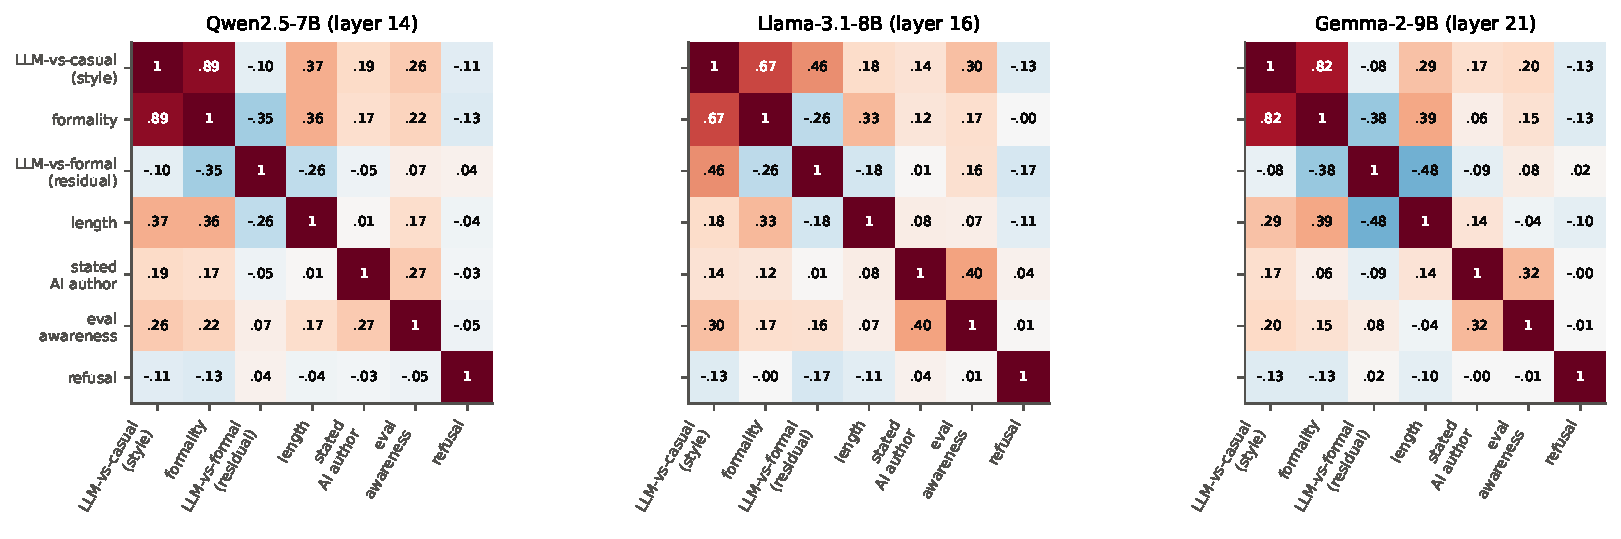
\includegraphics[width=\linewidth]{figs/cosines}
\caption{Cosine similarities between last-token difference-of-means directions at the steering layer.}
\label{fig:cos}
\end{figure}

Figure~\ref{fig:cos} shows cosines between directions at the steering layer. The style direction is close to the formality direction (0.89, 0.67, 0.82 for Qwen, Llama, Gemma) and far from the refusal direction ($-0.11$ to $-0.13$). The formality-matched residual direction is nearly orthogonal to the style direction in Qwen and Gemma ($-0.10$, $-0.08$) and moderately aligned in Llama (0.46). The style direction has small positive cosine with the stated-authorship direction (0.14--0.19) and with the evaluation-awareness direction (0.20--0.30); the latter two are more aligned with each other (0.27--0.40). The residual direction is orthogonal to both ($|\cos|\le 0.16$).

Projections tell the same story from the other side. In Qwen, the stated-authorship direction ``fires'' on LLM-style prompts (AUC 0.85 for LLM versus casual at short length, 0.97 at long length) and the evaluation-awareness direction does too (0.77, 0.88); but both fire equally on formal-human prompts (0.87 and 0.74 for formal versus casual) and neither separates LLM-style from formal-human prompts (0.47, 0.56). In Llama and Gemma these projections are weaker (0.51--0.68 for LLM versus casual). So, to the extent that an LLM-styled prompt looks more ``AI-authored'' or more ``evaluation-like'' to the model's own concept directions, it does so through formality. One caveat: our contrastive concept directions are only moderately consistent across the four phrasings used to build them (mean pairwise cosine 0.24--0.44).

\subsection{Steering with the text held fixed}
\label{sec:steer}

\begin{figure}[t]
\centering
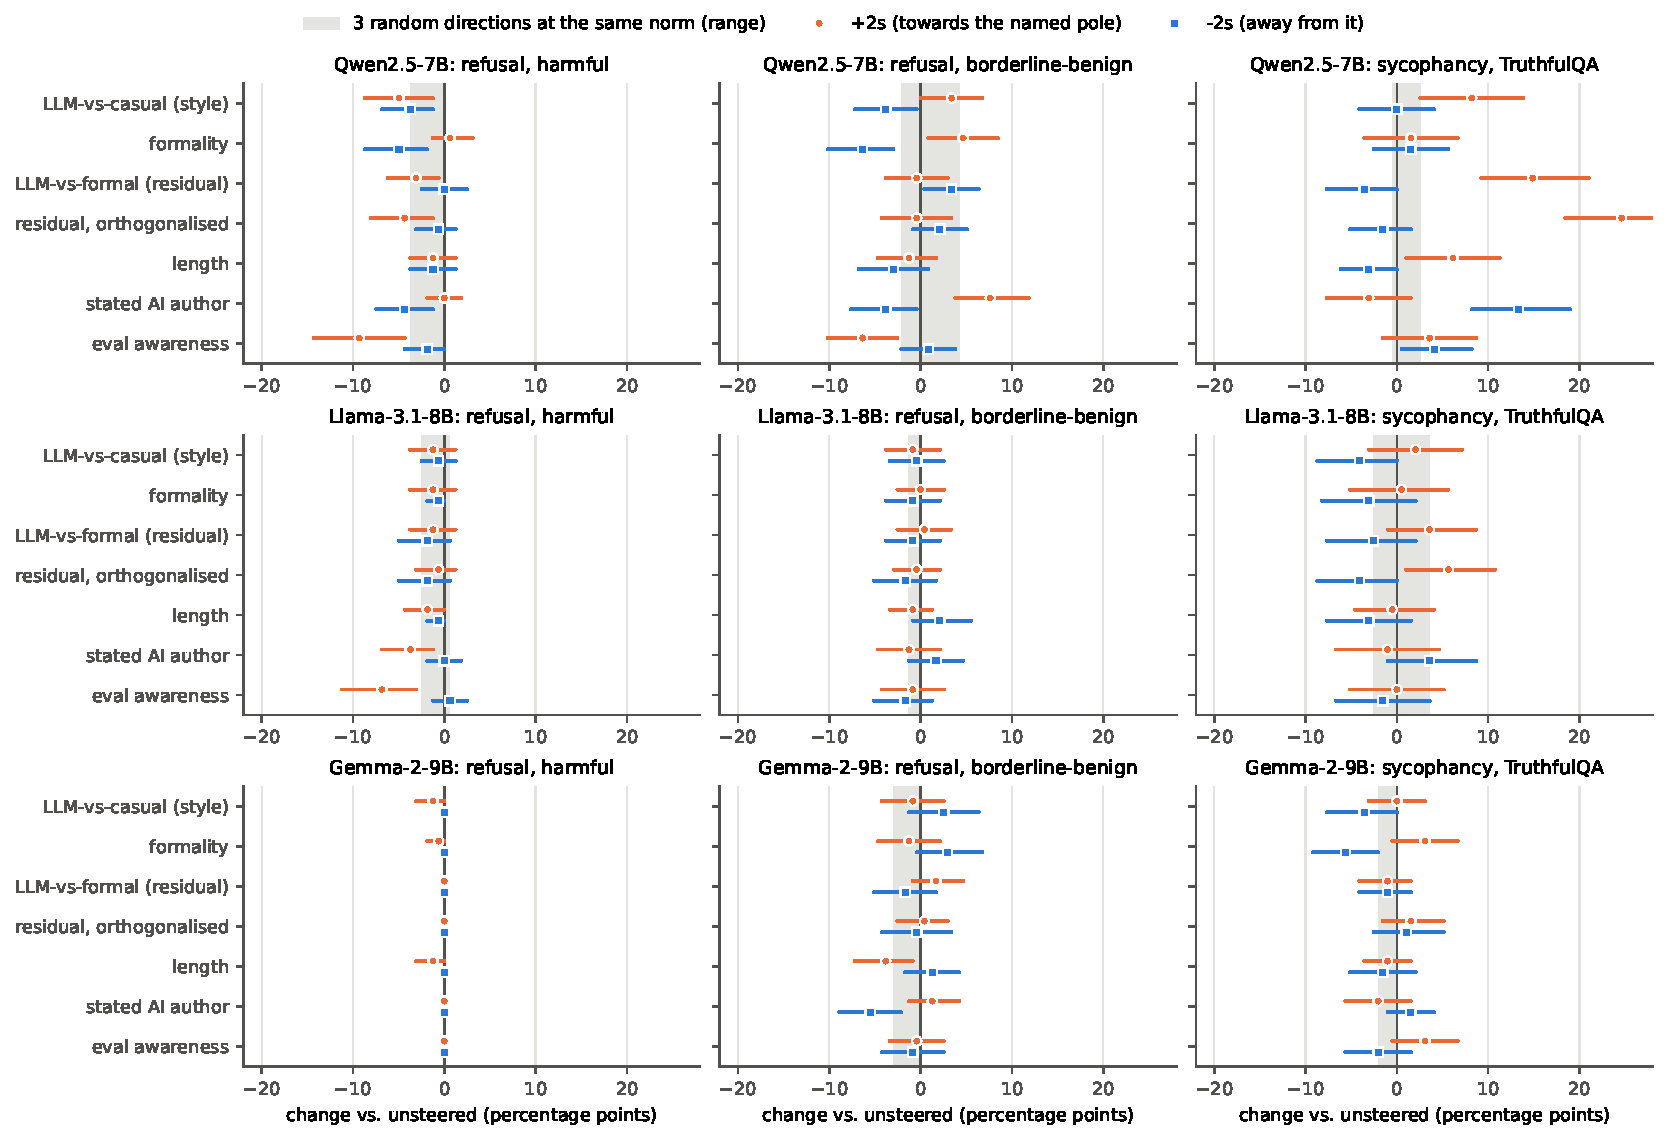
\includegraphics[width=\linewidth]{figs/steering}
\caption{Change in behaviour on the original human prompts when a direction is added at $\pm2s$ ($s$ = norm of the natural LLM-minus-casual gap at the steering layer). The grey band is the range of three random directions of the same norm. Intervals are 95\% item-bootstrap. The refusal direction (positive control, not shown) moves harmful refusal by $-39$/$-14$/$-3$ points at $-2s$ and borderline refusal by $+84$/$+25$/$+12$ points at $+2s$ in Qwen/Llama/Gemma.}
\label{fig:steer}
\end{figure}

\begin{figure}[t]
\centering
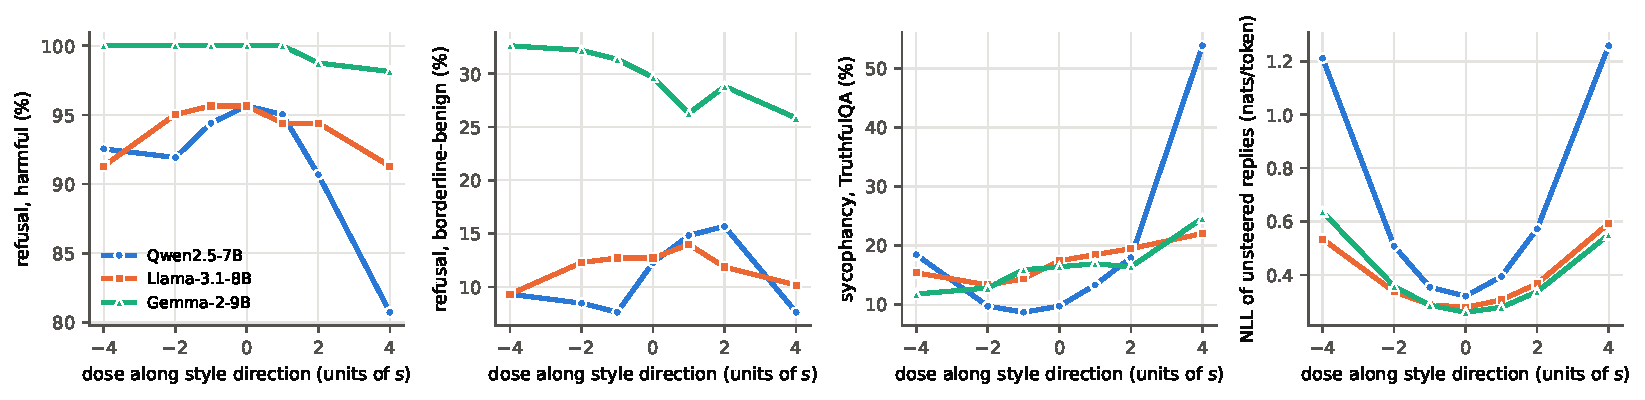
\includegraphics[width=\linewidth]{figs/dose}
\caption{Dose-response along the style direction. Behaviour is flat around the natural dose ($\pm1s$); larger doses mainly raise sycophancy and degrade the model (right panel).}
\label{fig:dose}
\end{figure}

\paragraph{The intervention reproduces the natural internal shift.} Adding $+1s$ of the style direction on casual prompts moves the downstream projection onto the style direction by 1.1--1.3 times the natural casual-to-LLM gap two layers later, and by 0.5--0.9 times at the final layer. Internally, the steered casual prompt therefore looks about as ``LLM-styled'' as a real LLM-styled prompt.

\paragraph{Natural dose: no detectable behavioural change.} At $+1s$, the changes in harmful refusal ($-0.6$, $-1.2$, $0.0$ points for Qwen, Llama, Gemma), borderline refusal ($+2.5$, $+1.3$, $-3.4$) and sycophancy ($+3.6$, $+1.0$, $+0.5$) all have intervals that include zero. At $-1s$ the only interval excluding zero is borderline refusal in Qwen ($-4.7$ $[-8.1,-1.3]$), which is of the same size as the spread of random directions at $2s$ in that model ($-2.1$ to $+4.2$). Degradation at $\pm1s$ is negligible ($\le 0.07$ nats per token).

\paragraph{Larger doses.} At $\pm2s$ (Figure~\ref{fig:steer}), Llama and Gemma remain within the random band on all three outcomes. In Qwen, $+2s$ raises sycophancy by 8.2 points $[+2.6,+13.8]$ (random: $-0.5$ to $+2.6$) and lowers harmful refusal by 5.0 points $[-8.7,-1.2]$ (random: $-0.6$ to $-3.7$). At $+4s$ sycophancy rises by 8.2 points in Gemma $[+4.1,+12.8]$ (random: $-0.5$ to $+1.5$) and by 44 points in Qwen, where however a random vector of that norm produces $+31$ and the likelihood of the model's own replies drops by about 0.9 nats per token. Across the three models the sycophancy curve is monotone in the dose (Figure~\ref{fig:dose}), with the same sign as the behavioural formal-versus-casual contrast: more formal/LLM-like means slightly more deference to the user's suggestion. The formality direction behaves like the style direction, as its cosine suggests (in Gemma, $-5.6$/$+3.1$ points of sycophancy at $\mp2s$). The formality-matched residual direction has no effect in Llama and Gemma; in Qwen it raises sycophancy at $+2s$ ($+14.9$; $+24.6$ after projecting out formality and length), but there $2s$ is about eight times that direction's natural norm.

\paragraph{Stated-authorship direction.} This direction is a working handle on the model's verbal authorship judgement: steering it from $-2s$ to $+2s$ moves the mean verbalised P(AI) for fixed casual prompts from 0.01 to 0.99 in Qwen (unsteered 0.24), from 0.08 to 0.18 in Llama and from 0.02 to 0.23 in Gemma, whereas the style direction barely moves it (Qwen 0.07 to 0.28; Llama 0.12 to 0.11; Gemma 0.06 to 0.05). Its behavioural effects in Qwen mirror the label experiment: $+2s$ raises borderline refusal by 7.6 points $[+3.8,+11.9]$, and $-2s$ (towards ``human'') raises sycophancy by 13.3 points $[+8.2,+19.0]$. In Gemma $-2s$ lowers borderline refusal by 5.5 points $[-8.9,-2.1]$. Llama shows no consistent effect. The evaluation-awareness direction at $+2s$ \emph{lowers} harmful refusal in Qwen ($-9.3$) and Llama ($-6.8$).

\paragraph{Within-item dose-response.} As a correlational complement, we ask whether items whose rewrite moved further along the style direction also changed behaviour more (Appendix~\ref{app:dose}). In Qwen no correlation differs from zero ($|r|\le0.10$). In Llama 2 of 10 are nominally significant. In Gemma 6 of 10 are, all small ($|r|$ between 0.10 and 0.16): larger shifts along the direction go with lower refusal and higher sycophancy, again the sign of the formality effect.

\subsection{Robustness}
With Gemini 2.5 Flash as the rewriter (Appendix~\ref{app:gemini}) the pattern is the same in the three open models: LLM minus formal-human is within $\pm1$ point on harmful refusal and $-0.4$ to $-3.3$ on borderline refusal (none significant); on sycophancy it is $-5.2$ $[-9.8,-1.0]$ in Qwen, $-3.6$ in Llama and $+2.6$ in Gemma, i.e.\ without a consistent sign. Elaboration again lowers harmful refusal ($-8.3$, $-6.9$, $-5.5$; all significant) and formal minus casual is again negative on harmful refusal ($-6.7$, $-4.5$, $-2.2$). With the second sycophancy judge, base rates are roughly twice as high but the LLM-minus-formal contrast remains null ($-0.5$, $-1.5$, $+3.6$; Appendix~\ref{app:judge}).
